\section{Introduction}
In previous chapters, we saw various examples of the combinational circuits and sequential circuits. In combinational circuits, the output depends on the current values of inputs only; whereas in sequential circuits, the output depends on the current values of the inputs along with the previously stored information. In the other words, storage elements, e.g. flip flogs or registers, are required for sequential circuits. 

The information stored in the these elements can be seen as the states of the system. If a system transits between finite number of such internal states, then finite state machines (FSM) can be used to design the system. In this chapter, various finite state machines along with the examples are discussed. 

\section{Comparison: Mealy and Moore designs}
FMS design is known as Moore design if the output of the system depends only on the states (see Fig. \ref{fig:MooreEdgeDetector}); whereas it is known as Mealy design if the output depends on the states and external inputs (see Fig. \ref{fig:MealyEdgeDetector}). Further, a system may contain both types of designs simultaneously. Following are the few differences in Mealy and Moore design, 


\begin{enumerate}
	\item In Mealy machine, the output is available as soon as the input is changed, whereas in Moore machine, the output is available after 1 clock cycle as shown in Fig. \ref{fig:edgeDetectorWave}.

	\item Mealy machine requires fewer number of states as compared to Moore machine as shown in Listing \ref{vhdl:edgeDetector}. 
	
	\item Mealy machines are good for synchronous systems as discussed in the chapter, but careful design is required for asynchronous systems. Therefore, Mealy machine can be complex as compare to Moore machine. 
\end{enumerate}

\section{Example: Rising edge detector}
Rising edge detector generates a tick for the duration of one clock cycle, whenever input signal changes from 0 to 1. In this section, state diagrams of rising edge detector for Mealy and Moore designs are shown. Then rising edge detector is implemented using VHDL code. Also, outputs of these two designs are compared. 

\subsection{State diagrams: Mealy and Moore design}
Fig. \ref{fig:MealyEdgeDetector} and \ref{fig:MooreEdgeDetector} are the state diagrams for Mealy and Moore designs respectively. In Fig. \ref{fig:MealyEdgeDetector}, the output of the system is set to 1, whenever the system is in the state `zero' and value of the input signal `level' is 1; i.e. output depends on both the state and the input. Whereas in Fig. \ref{fig:MooreEdgeDetector}, the output is set to 1 whenever the system is in the state `edge' i.e. output depends only on the state of the system. 

\begin{figure}[h!]
	\centering
	\begin{subfigure}[t]{0.5\textwidth}
		\centering
		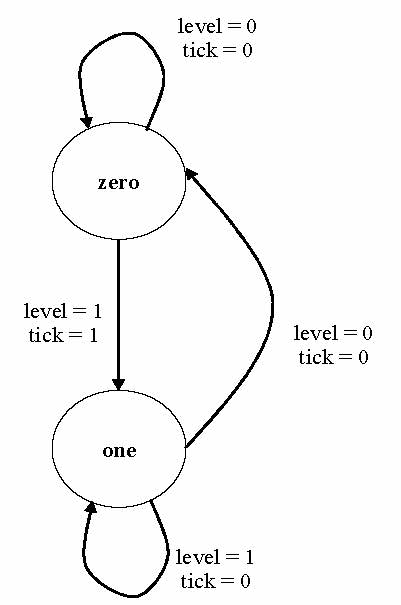
\includegraphics[scale=1]{MealyEdgeDetector}
		\caption{Mealy Design}
		\label{fig:MealyEdgeDetector}
	\end{subfigure}%
	\begin{subfigure}[t]{0.5\textwidth}
		\centering
		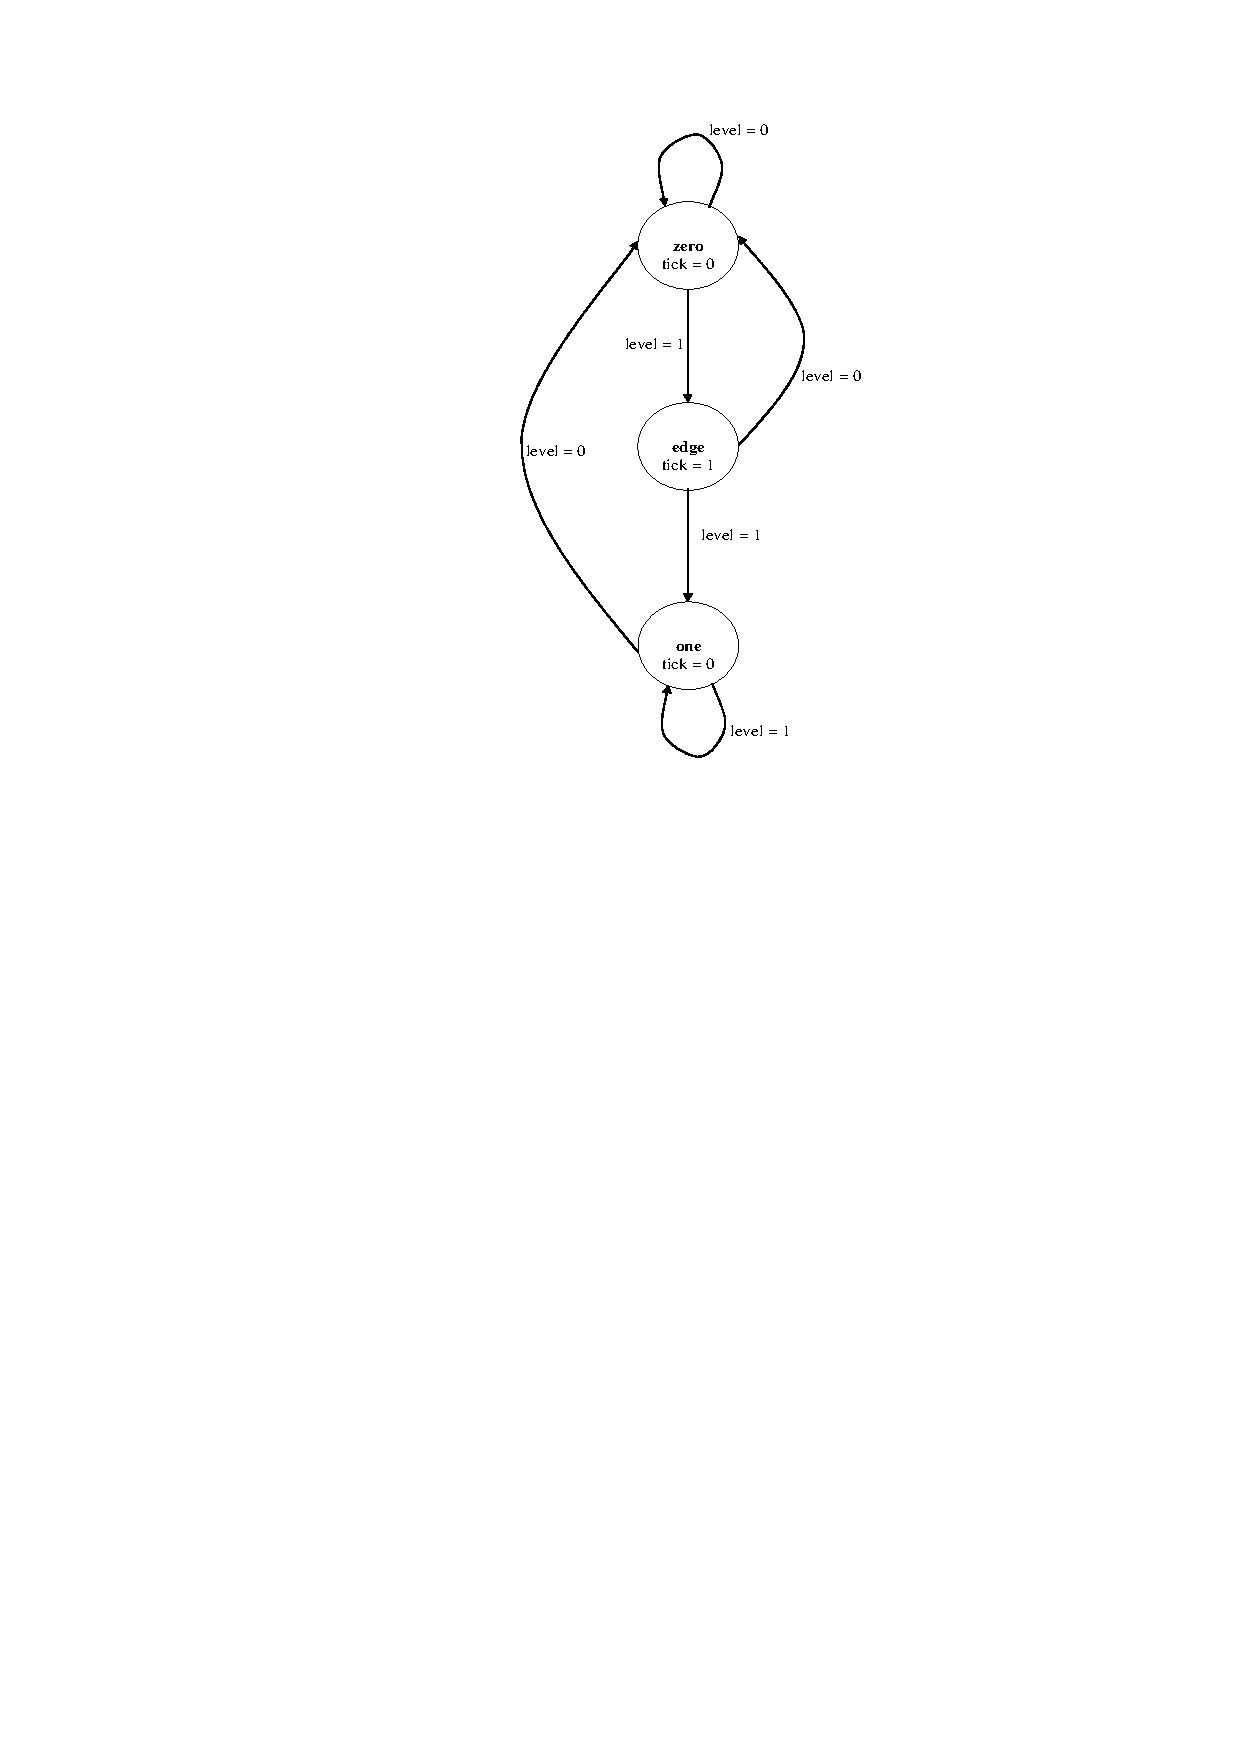
\includegraphics[scale=0.8]{MooreEdgeDetector}
		\caption{Moore Design}
		\label{fig:MooreEdgeDetector}
	\end{subfigure}
	
	\caption{State diagrams for Edge detector }
\end{figure}


%\begin{figure}[!h]
%	\centering
%	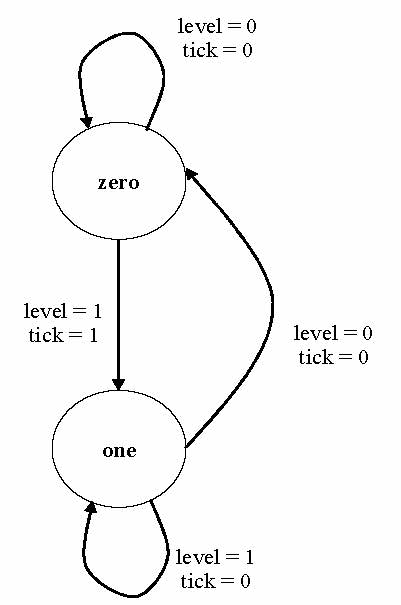
\includegraphics[scale=1]{MealyEdgeDetector}
%	\caption{Edge Detector with Mealy Design}
%	\label{fig:MealyEdgeDetector}
%\end{figure}
%
%\begin{figure}[!h]
%	\centering
%	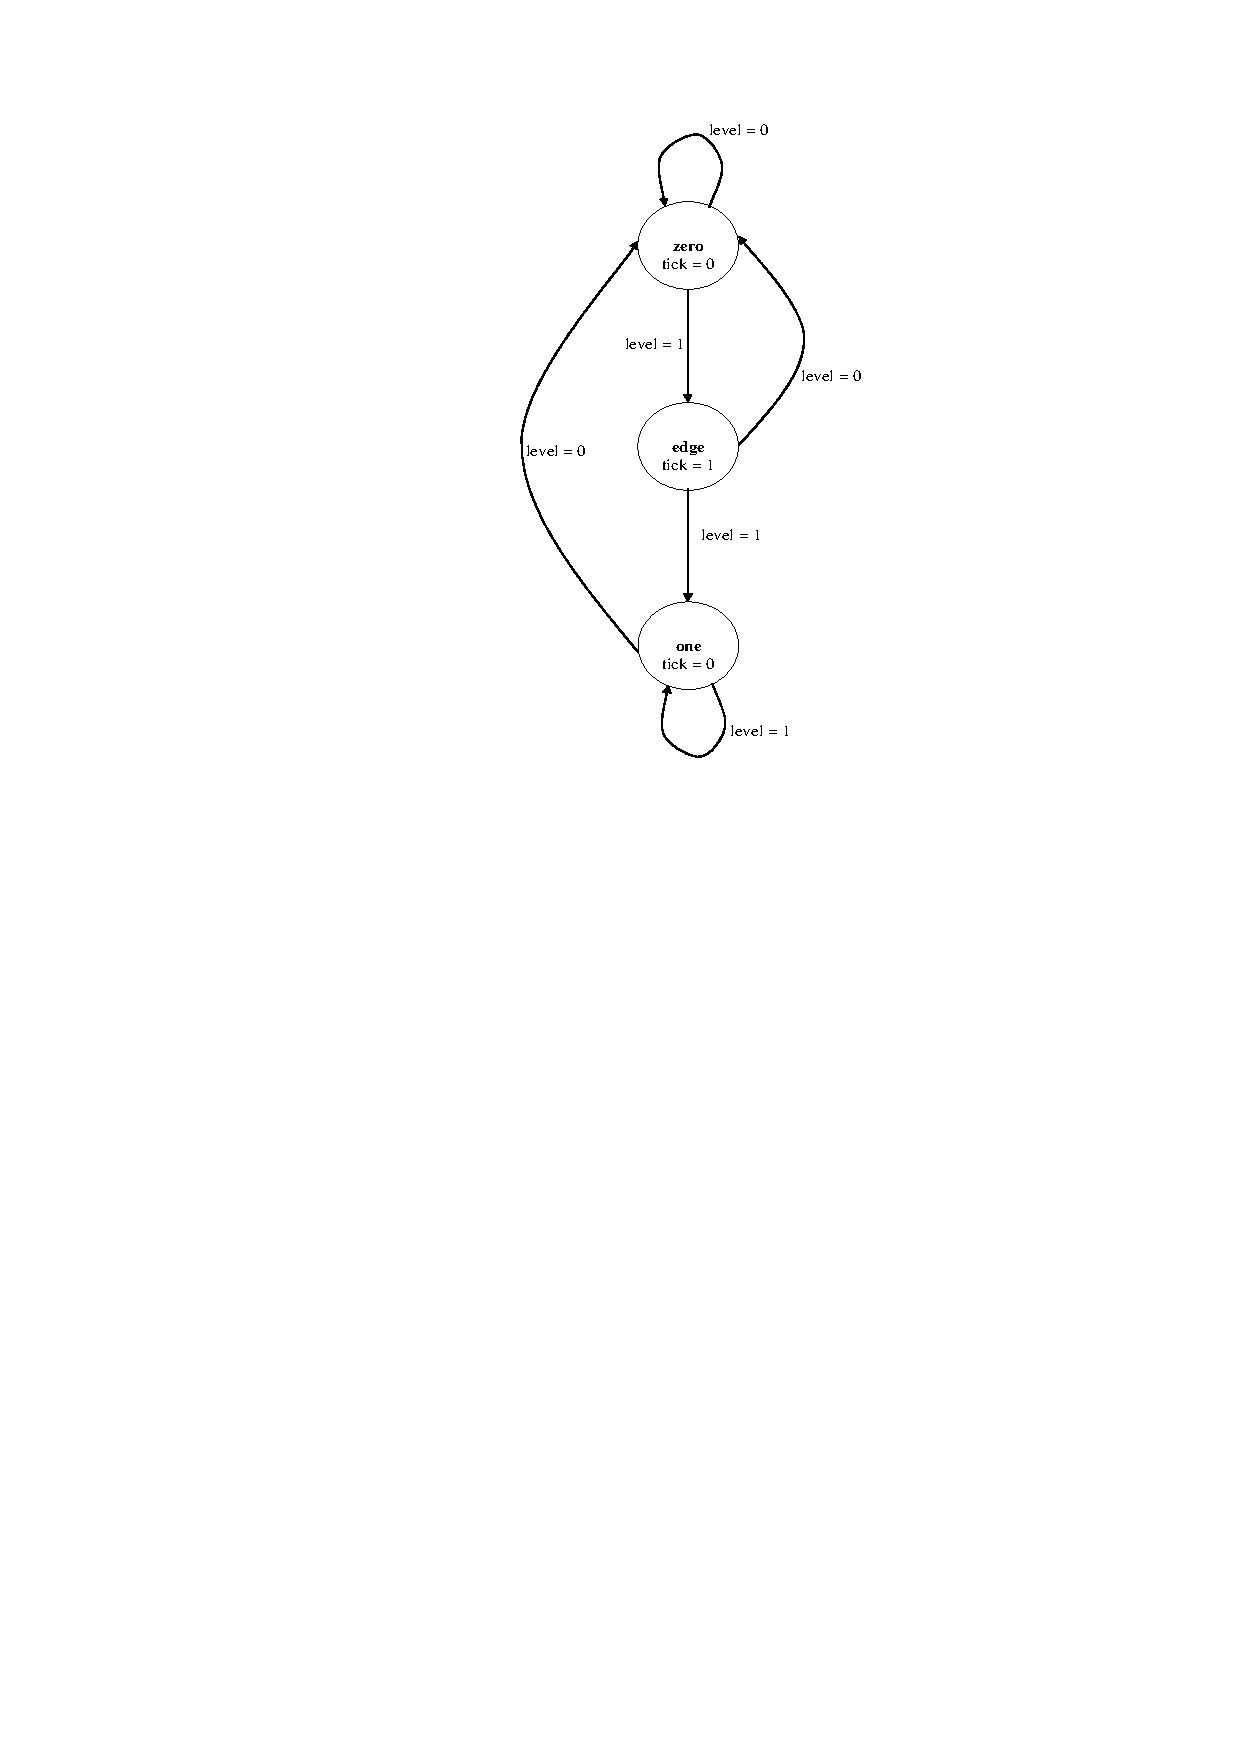
\includegraphics[scale=0.8]{MooreEdgeDetector}
%	\caption{Edge Detector with Moore Design}
%	\label{fig:MooreEdgeDetector}
%\end{figure}


\subsection{Implementation}
Both Mealy and Moore designs are implemented in Listing \ref{vhdl:edgeDetector}. The listing can be seen as two parts i.e. Mealy design (Lines 36-54) and Moore design (Lines 56-80). Please read the comments for complete understanding of the code. The simulation waveforms i.e. Fig. \ref{fig:edgeDetectorWave} are discussed in next section. 
\lstinputlisting[
language = Vhdl,
caption    = {Edge detector: Mealy and Moore designs},
label      = {vhdl:edgeDetector}
]{edgeDetector.vhd}

\subsection{Outputs comparison}

In Fig. \ref{fig:edgeDetectorWave}, it can be seen that output-tick of Mealy detector is generated as soon as the `level' goes to 1, whereas Moore design generate the tick after 1 clock cycle. These two ticks are shown with the help of the two red cursors in the figure. Since, output of Mealy design is immediately available therefore it is preferred for synchronous designs. 

\begin{figure}[!h]
	\centering
	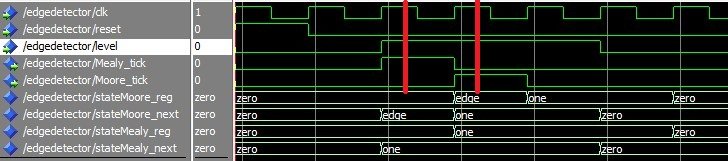
\includegraphics[width=\textwidth]{edgeDetectorWave}
	\caption{Simulation waveforms of rising edge detector in Listing \ref{vhdl:edgeDetector}}
	\label{fig:edgeDetectorWave}
\end{figure}

\subsection{Visual verification}
Listing \ref{vhdl:edgeDetector_VisualTest} can be used to verify the results on the FPGA board. Here, clock with 1 Hz frequency is used in line 19, which is defined in Listing \ref{vhdl:clockTick}. After loading the design on FPGA board, we can observe on LEDs that the output of Moore design displayed after  Mealy design, with a delay of 1 second.  

\lstinputlisting[
language = Vhdl,
caption    = {Visual verification of edge detector},
label      = {vhdl:edgeDetector_VisualTest}
]{edgeDetector_VisualTest.vhd}

\section{Conclusion}
In this chapter, Mealy and Moore designs are discussed. Also, `edge detector' is implemented using Mealy and Moore designs. This example shows that Mealy design requires fewer states than Moore design. Further, Mealy design generates the output tick as soon as the rising edge is detected; whereas Moore design generates the output tick after a delay of one clock cycle. Therefore, Mealy designs are preferred for synchronous designs. 